\section{Feature Representation Learning}
\label{feature-learning:sec}

\begin{figure}[t]
	\centering
	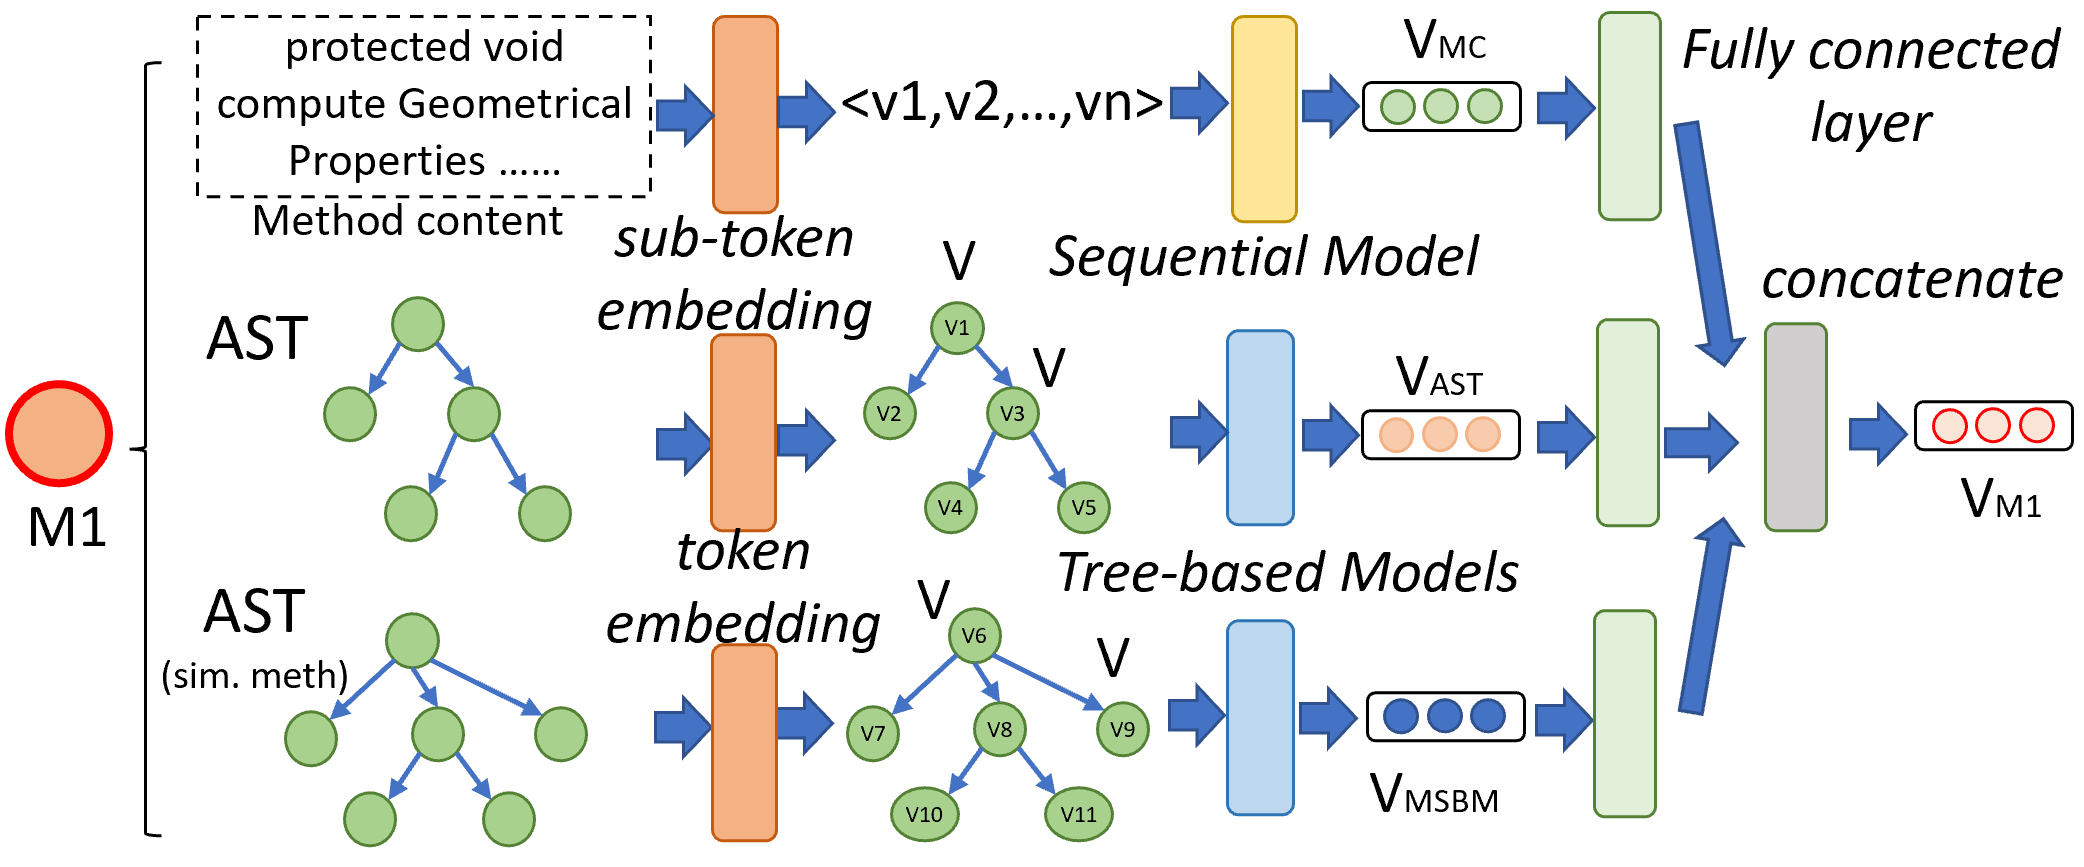
\includegraphics[width=3.4in]{graphs/step-2-method-new.png}
	\caption{Method-level Feature Representation Learning}
	\label{method-level-feature-learning}
\end{figure}


\begin{figure}[t]
	\centering
	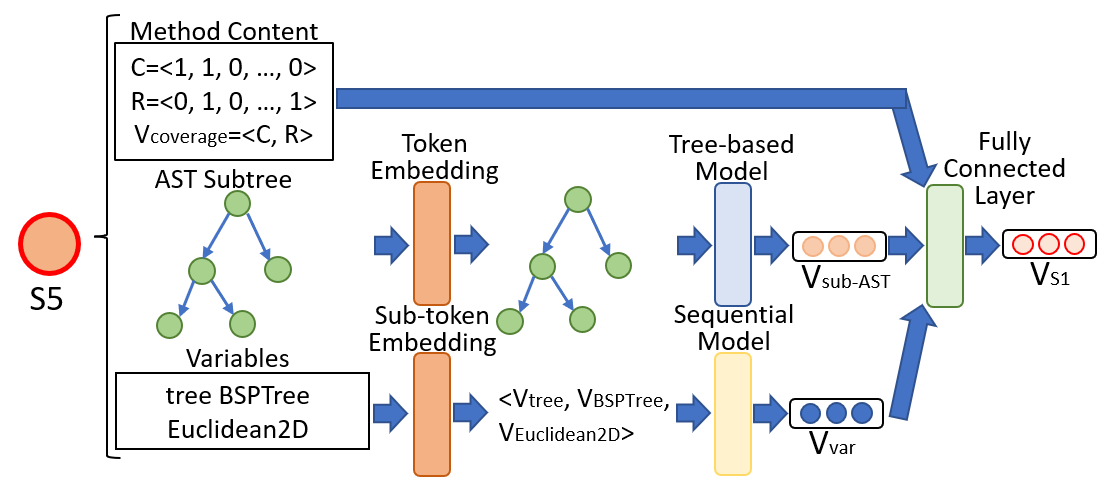
\includegraphics[width=3.4in]{graphs/step-2-statement-new.png}
	\caption{Statement-level Feature Representation Learning}
	\label{statement-level-feature-learning}
\end{figure}

In this step, \tool aims to learn the node feature embeddings based on the node features generated from step 1. So the input of this step is the method-level and statement-level graphs, and the expected output is the node embedding vectors for each node in each graph.

To be more in detail, we introduce the node feature representation learning also from both method-level and statement-level.

\subsection{Method-level Feature Representation Learning}

From step 1, for each node that represent a method $m$, there are extracted sequence of sub-tokens $Seq^p_m$ as the method content, generated AST $Tree_m$, and the generated AST $$

{\bf As for the Method-Level:}
\begin{itemize}
	\item Method Content: \tool has the processed sequence of sub-tokens $Seq^p_m$ from the last step. In this step, \tool uses the GloVe \cite{pennington2014glove} to learn the sub-token embedding and then replace each sub-token with the embedding vector generated from GloVe. After the replacement, \tool has a sequence of vector $Seq^{pe}_m$ and then uses a GRU layer \cite{cho2014learning} to learn the embedding vector $vec_{mc}$ for the method content. 
	
	\item Method Structure: \tool has the generated AST $Tree_m$ from the last step. In this step, \tool also firstly uses the GloVe to vectorize the AST and then uses a deep learning-based model TreeCaps \cite{bui2021treecaps} to learn the embedding vector $vec^{ms}$.
	
	\item Similar Buggy Method: \tool has the most similar buggy method $m_b$ from the last step. In this step, \tool has the same process as the method structure feature by using the GloVe and TreeCaps to learn the embedding vector $vec^{sbm}$.
\end{itemize}

{\bf As for the Statement-Level:}
\begin{itemize}
	\item Code Coverage Information: \tool has the code coverage information $C = <c_1, c_2, ..., c_i>$ from last step. In this step, \tool does not make any changes and directly regard $C$ as the embedding vector $vec_{cci}$ for the code coverage information.
	
	\item Statement Structure: \tool has the generated sub-AST $Tree_s$ from the last step. In this step, \tool does a similar process as the method-level by firstly using the GloVe to vectorize the AST and then using a deep learning-based model TreeCaps to learn the embedding vector $vec^{ss}$.
	
	\item Variables: \tool has the variable sequence with variable types $Seq_s$ from the last step. In this step, \tool uses the GloVe to learn the token (here can be the variable name and variable type) embedding and then replace each token with the embedding vector generated from GloVe. And then, \tool uses one GRU layer to learn the embedding vector $vec_{v}$ for the whole variable information sequence $Seq_s$
\end{itemize}

After having the six embedding vectors mentioned above, \tool uses six fully connected layers to standardize each embedding vector's length to $l/3$ (Here l/3 is an integer). And then, for both method-level and statement-level, \tool concatenate three feature embedding vector into one vector $vec_{m}$ or $vec_{s}$ for the method-level or statement-level with the length of $l$. In this case, for both method-level and statement-level, \tool all has a combined graph $G_m$ or $G_s$ with the node embedding vector $vec_{m}$ or $vec_{s}$. It is the input for the next step.